\documentclass[openany]{book}


%Standard Stefanos Packages
\usepackage[utf8]{inputenc}
\usepackage{dirtytalk}
\usepackage{amsmath}
\usepackage{mathtools}  
\mathtoolsset{showonlyrefs} 
\usepackage{graphicx}
\usepackage{mdframed}
\usepackage{lipsum}
\usepackage{cancel}
\usepackage{systeme}
\usepackage{pgfplots}
\usepackage{textcomp}
\usepackage{geometry}
\usetikzlibrary{arrows}
\geometry{a4paper}
\graphicspath{ {./res/} }
\usepackage{float}
\restylefloat{table}
\newcommand{\comment}[1]{%
	\text{\phantom{(#1)}} \tag{#1}
}
 \title{\line(3,0){250}\\Data Science Algorithms and Tools \\ Coursework 1  \\\line(3,0){250}}
\usepackage{pgfplots}
\newmdtheoremenv{note}{Note}
\pgfplotsset{compat=1.17}


%Extra Packages
\usepackage{tikz}
\usepackage{subcaption} 
\usetikzlibrary{automata,positioning}

\usepackage{listings}
\usepackage{xcolor}

\definecolor{dkgreen}{rgb}{0,0.6,0}
\definecolor{gray}{rgb}{0.5,0.5,0.5}
\definecolor{mauve}{rgb}{0.58,0,0.82}

\lstdefinestyle{myScalastyle}{
	frame=tb,
	language=scala,
	aboveskip=3mm,
	belowskip=3mm,
	showstringspaces=false,
	columns=flexible,
	basicstyle={\small\ttfamily},
	numbers=none,
	numberstyle=\tiny\color{gray},
	keywordstyle=\color{blue},
	commentstyle=\color{dkgreen},
	stringstyle=\color{mauve},
	frame=single,
	breaklines=true,
	breakatwhitespace=true,
	tabsize=3,
}



\begin{document}
	\maketitle
	\chapter{Task 1:Clustering}
		\section{Without Normalization}
			\subsection{Compare KMeans Clastering results with reference labels}
				As we can see, the clustering is not perfect; there is a significant amount of points classified as being in a different class than expected.
				However, something that is expected to some degree is due to the nature of the k-means algorithm to work with centroids. Points that are closer
				to a cluster of a different label(within-cluster outliers) have a high chance of being classified on the wrong cluster. Another potential source of error in our setup is the 
				the fact that currently, we do not perform normalization. PCA is a maximize-variance technique; by not normalize our data with 
				the max values in mind, we significantly undermine the Clustering solution performance, as no normalized data do not have any upper 
				limit on the values of their individual features.
				\begin{figure}[H]
					\iftrue
					\centering
					\caption{a}
					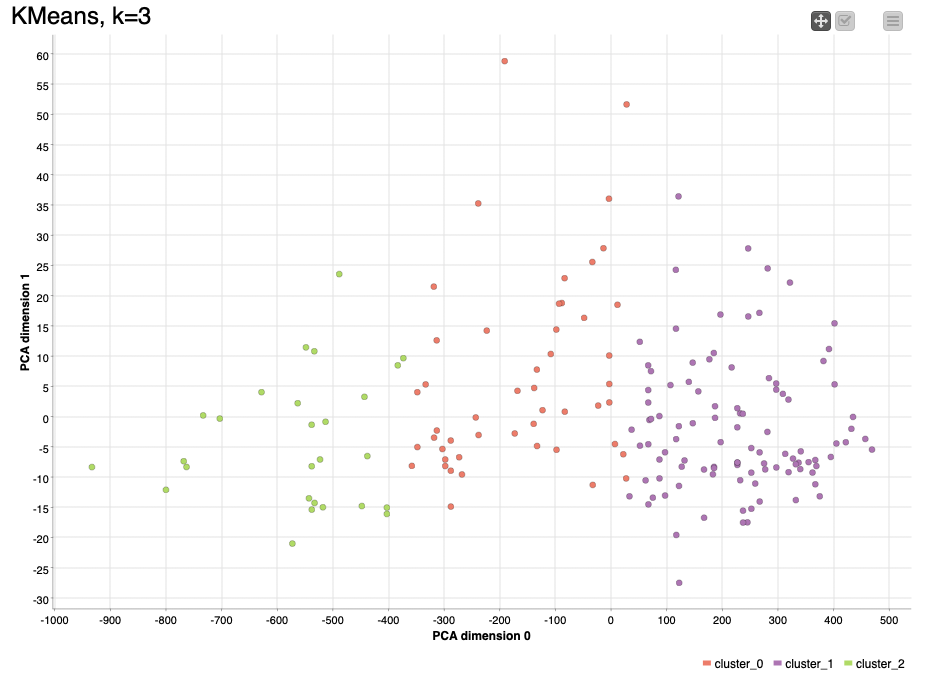
\includegraphics[scale=0.3]{res/task1.1.kmeans}
					\fi
				\end{figure}
				\begin{figure}[H]
					\iftrue
					\centering
					\caption{b}
					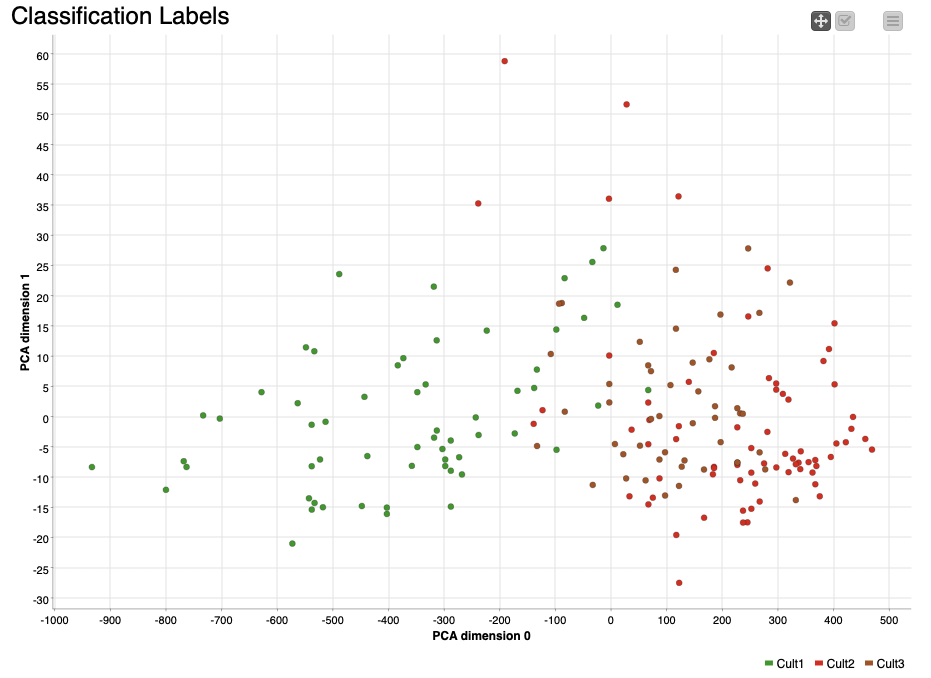
\includegraphics[scale=0.3]{res/task1.1.nokmeans}
					\fi
				\end{figure}
			\subsection{Cluster Validity Measure, WSS/BSS}
				\subsubsection{Explanation of Validity Measure chosen}
					The WSS/BSS cluster validity measure was used to determine the quality of the solution.
					The Within-Cluster Sum of Squares(WSS) represents how closely related are the objects(Square deviations of every point from centroid) within every cluster.
					\begin{equation}
						\sum_{i}^{}\sum_{x\in{C_i}}^{}{(x-m_{i})^2}
					\end{equation}
					Where the Between-Cluster sum of Squares(BSS) represents how closely related are the clusters themselfs(deviations of cluster centroids from the centroids-centroid) 
					\begin{equation}
						\sum_{i}^{}{|C_i|(m-m_{i})^2}
					\end{equation}
					Where $|C_i|$ is the size of cluster $i$, $m_i$ is the cluster mean and $m$ is the overall mean
					\begin{figure}[H]
						\iftrue
						\centering
						\caption{b}
						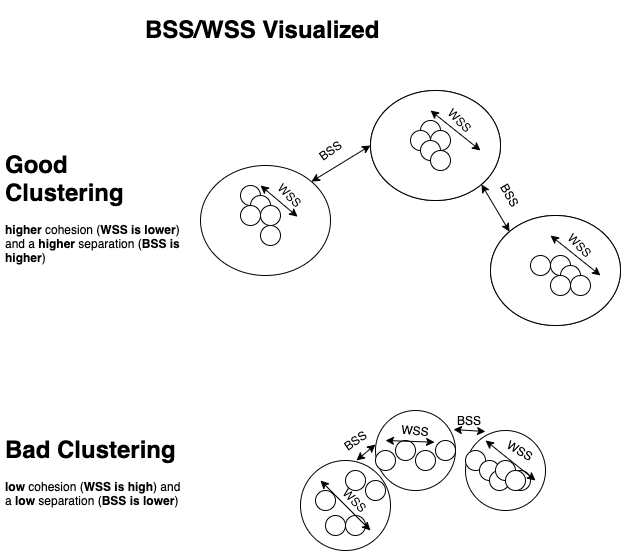
\includegraphics[scale=0.3]{res/bss-wss}
						\fi
					\end{figure}
				\subsubsection{Comments on results}
					\begin{itemize}
						\item WSS : 2630540.93174603
						\item BSS : 1.4958714555014689E7
					\end{itemize}
					Our BSS is significantly bigger than WSS, meaning that our clustering solution is sufficient in terms of this metrics. High cohersion(low WSS)
					and high separation (High BSS) makes sure that our clusters are well centered into their centroids, and the centroids are further apart so 
					the probability of a given datapoint to be classified wrongly is small. 
		\section{With Normalization}
			\subsection{Compare KMeans Clastering results with reference labels}
				As we can see, the clustering solution here is way better, this is due to the fact that PCA performed way better, revealing the data's well separated
				nature. We can see and verify that the number of false-positives are smaller than before.
				\begin{figure}[H]
					\iftrue
					\centering
					\caption{a}
					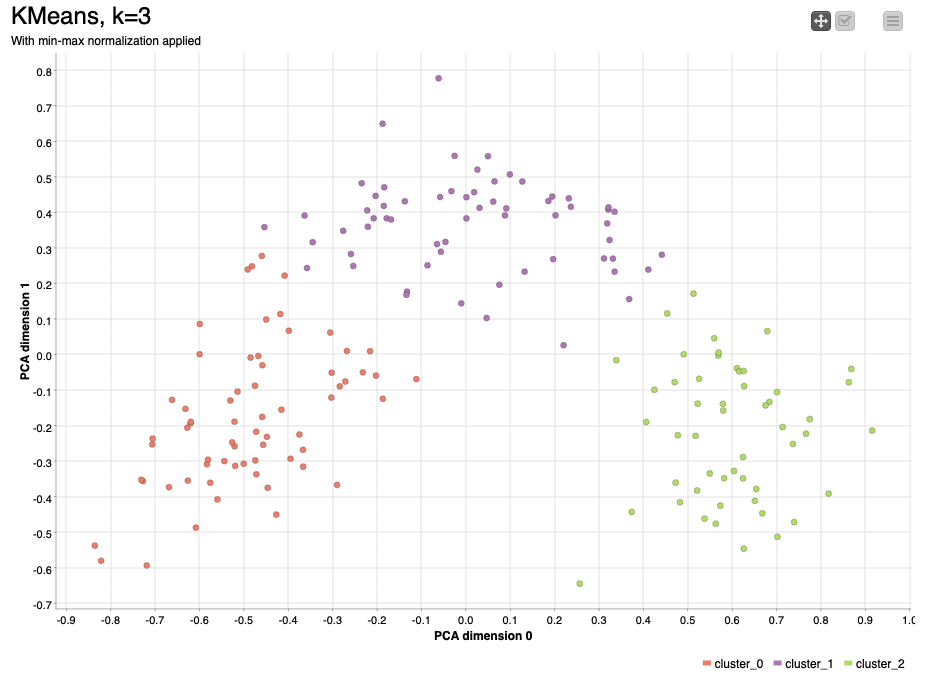
\includegraphics[scale=0.3]{res/task1.2.kmeans}
					\fi
				\end{figure}
				\begin{figure}[H]
					\iftrue
					\centering
					\caption{b}
					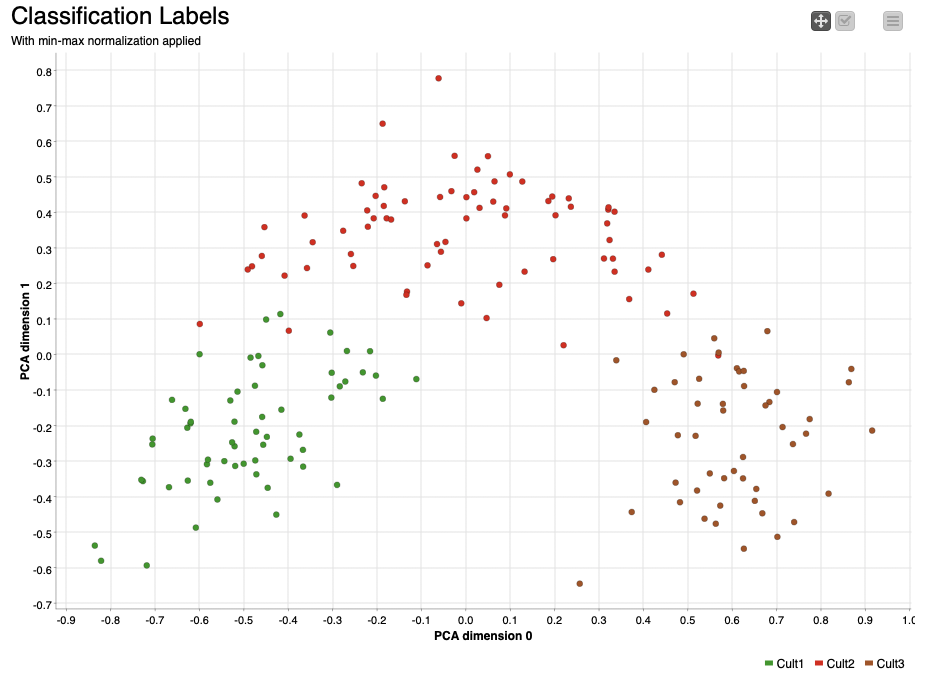
\includegraphics[scale=0.3]{res/task1.2.nokmeans}
					\fi
				\end{figure}
			\subsubsection{Comments on results}
				\begin{itemize}
					\item WSS : 10.77176280410001
					\item BSS : 46.32012470161712
				\end{itemize}
				Again, our BSS is significantly bigger than WSS, meaning that our clustering solution is sufficient in terms of these metrics. High cohesion(low WSS)
				and high separation (High BSS) makes sure that our clusters are well centered into their centroids, and the centroids are further apart so 
				the probability of a given data point being classified wrongly is small. However, how can we compare the two aforementioned clustering solutions?
			\subsubsection{Entropy and Quality}
				To be able to objectively compare our K-Means results, it is nessesary to introduce two new metrics.
				Entropy H is defined as
				\begin{equation}
					H=-\sum_{0}^{n}{p_i\log(p_i)}
				\end{equation}
				Entropy describes the amount of pure information, that is contained into a probabilistic system.
				
				Quality of a clustering solution, is defined as
				\begin{equation}
					Q=1-E_{norm}, 0\leq Q \leq 1
				\end{equation}
				Where $E_{norm}$ is the Sum of normalized entropy of every cluster. Lets compare our clustering solutions,
				with and without normalisation as a pre-proccesing step
				\begin{table}[H]
					\centering
					\begin{tabular}{ll}
						Q\_norm & Q\_raw \\
						0.839   & 0.405 
					\end{tabular}
				\end{table}
				As we can see, our clustering solution performs better with the normalization part enabled.
	\chapter{Task 2:Classification}
		\section{(NNC)NN Classifier}
			The Nearest Neighborhood algorithm is a simple geometric method to classify unlabelled data. NN-Classification does not create a model of the information
			rather uses the training data to estimate the class of the new data. Let $s$ to be the new unlabelled datapoint in 2 dimensions, and the labelled training datapoints $v_1,v_2...v_k$.
			\begin{figure}[H]
				\iftrue
				\centering
				\caption{b}
				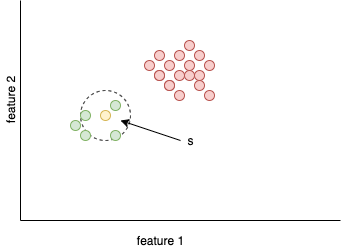
\includegraphics[scale=0.5]{res/nn}
				\fi
			\end{figure}
			By taking the n closest neighbors of the given data point and examining their classes from the training dataset, we can determine the class of our unlabelled datapoint.
			This method is extremely powerful yet slow(as the whole training dataset is used per query) and can be easily fooled by noisy data.
		\section{(DTC)Desision Tree Classifier}
			Decision Trees, on the other hand, create an explicit model of the data and tries to predict future observations using only the model above. The Decision trees create
			a dynamic tree of decision criteria that can be associated with a particular label. Let the following five rows from the famous iris dataset.
			\begin{table}[H]
				\centering
				\begin{tabular}{lllll}
					Sepal Length & Sepal Width & Petal Length & Petal Width & Class Label     \\
					4.9 & 3.0 & 1.4 & 0.2 & Iris-setosa     \\
					7.0 & 3.2 & 4.7 & 1.4 & Iris-versicolor \\
					6.4 & 3.2 & 4.5 & 1.5 & Iris-versicolor \\
					5.9 & 3.0 & 5.1 & 1.8 & Iris-virginica 
				\end{tabular}
			\end{table}
			A Decision Tree Classifier will associate feature value ranges to different class labels. From the aforementioned table, we can observe the following facts.
			\begin{itemize}
				\item if (Sepal Width==3.0) then Iris-versicolor, else if > 3.0, then Iris-setosa or Iris-virginica
				\item if (Sepal Length between 5.9 - 6.4) then Iris-virginica
				\item if (Sepal Length <5.9) then Iris-setosa
			\end{itemize}
			The following decision tree will match this facts.
			\begin{figure}[H]
				\iftrue
				\centering
				\caption{b}
				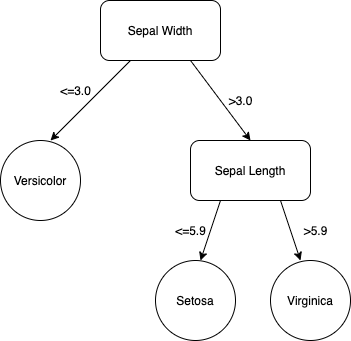
\includegraphics[scale=0.5]{res/dt}
				\fi
			\end{figure}

		\section{k-fold validation and scorer}
			For the training of both the classification algorithms, the k-fold algorithm is used. Under this algorithm, there are several 
			iterations, k. and every iteration, the training data set gets separated into k-1 training sets and 1 test set. Then the training is complete,
			the algorithm gets tested using the k*1=k test tests, and the accuracy and error rates are computed from those sets. The following diagram visualizes the process.
			\begin{figure}[H]
				\iftrue
				\centering
				\caption{b}
				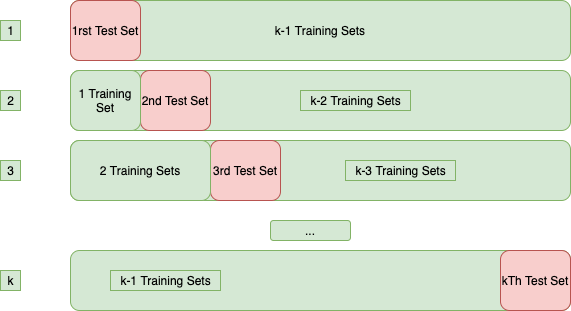
\includegraphics[scale=0.5]{res/kfold}
				\fi
			\end{figure}
		\section{Results}
			The following results were aquired with the following hyperparameters
			\begin{itemize}
				\item NN Classifier, 5 Weighted by distance closest neighboors
				\item Desision tree classifier with min number of records per node=4 
			\end{itemize}
			\begin{table}[H]
				\centering
				\begin{tabular}{ll}
					NNC Error & DTC Error \\
					23.2\%   & 8.9\%
				\end{tabular}
			\end{table}
			Found after extensive tuning of the hyperparameters, taken into account the risk of overfitting for DTC, and noice/faraway/irrelevant datapoints distraction for NNC. 
			
			
			
		
	
			
			
		
\end{document}